\documentclass[10pt]{article}
\usepackage[left=3.3cm,right=3.3cm,bottom=3.0cm,top=3.0cm]{geometry}
\usepackage{float}
\usepackage{graphicx}
\usepackage{tikz}
%\usepackage{amsthm}

\usetikzlibrary{arrows}

%\theoremstyle{definition}
%\newtheorem{definition}{Definition}

\newcommand{\LengthVar}{L}
\newcommand\Base[1]{{\tt #1}}
\newcommand{\ReadArrowType}{latex}

\title{A Bidirected String Graph Model for Genome Assembly}
\author{Eric Biggers}

\begin{document}
\maketitle

%\begin{abstract}
%Sequencing an organism's genome is an important step to further genetic research
%on that organism.  However, current sequencing machines can only sequence very
%short fragments of DNA that originate from random positions on the original
%genome, assembly software such as Allpaths-LG can be used to assemble these
%fragments into longer contiguous sequences.  
%\end{abstract}

\section{Introduction to genome sequencing and assembly}

\subsection{Definition of a genome}

Every living organism contains a collection of hereditary material called a {\em
genome}.  Typically, each cell of a multicellular organism contains a complete
copy of that organism's genome.  A genome consists of one or more DNA ({\it
deoxyribonucleic acid}) molecules in the form of {\it chromosomes}.  DNA is a
double-stranded molecule, each strand of which is a polymer of {\em
nucleotides}.  A nucleotide, together with the corresponding nucleotide on the
opposite strand, is called a {\it base pair} (abbreviation: {\it bp}).  In DNA,
there are four possible nucleotides: adenine, cytosine, guanine, and thymine,
which are abbreviated as \Base{A}, \Base{C}, \Base{G}, and \Base{T},
respectively.  \Base{A} always pairs with T on the other strand, and \Base{C}
always pairs with \Base{G} on the other strand.  In addition, each strand has a
direction, and the two strands of a DNA molecule are directed opposite one
another.  Furthermore, a DNA molecule may be circular, as is usually the case
for bacterial chromosomes.

Based on these biological facts, a genome is formally defined, for the purposes
of this paper, as a set of possibly circular, dual-stranded strings of the
symbols \Base{A}, \Base{C}, \Base{G}, and \Base{T}, where dual-stranded has the
meaning indicated above: the two strands run in opposite directions, and the
pairings \Base{A}---\Base{T} and \Base{C}---\Base{G} always hold.

This definition does not account for the fact that the genomes of diploid and
polyploid organisms, including most plants and animals, contain multiple
slightly-differing copies of each chromosome.  In this case, the above
definition will consider each copy of each chromosome to be a completely
different string in the genome, unless the copies are completely identical.

Genomes vary widely in size, from several thousand base pairs to many billion
base pairs, depending on the organism (see Table \ref{tab:GenomeSizes}).

\begin{table}[H]
	\begin{center}
		\begin{tabular}{|l|p{4.5cm}|}
			%\hline
			%$\phi$X174 bacteriophage &  $\sim$5,000 bp \\
			%\hline
			%Human mitochondrion &  $\sim$16,000 bp \\
			\hline
			{\bf Organism} & {\bf Approximate genome size (in base
			pairs)} \\
			\hline
			{\it Variola} virus (smallpox) &  186,000 \\
			\hline
			{\it E. coli} (a bacterium) & 4,600,000 \\
			\hline
			{\it Ananas comosus} (domesticated pineapple) & 500,000,000 \\
			\hline
			{\it Zea mays} (domesticated corn) & 2,000,000,000 \\
			\hline
			{\it Homo sapiens} (human)       &  3,200,000,000 \\
			\hline
		\end{tabular}
	\end{center}
	\caption{Approximate genome sizes of selected organisms}
	\label{tab:GenomeSizes}
\end{table}

\subsection{Genome sequencing}

{\it DNA sequencing} is the process of determining the base pair sequence of
({\it sequencing}) one or more DNA molecules.  {\it Genome sequencing} is the use
of DNA sequencing to determine the base pair sequence of an entire genome.

Sequencing a DNA molecule is very difficult because it is in fact an actual
molecule, which makes each base pair much too small to be directly observed.
Therefore, indirect laboratory techniques must be used.  Advances in these
techniques are progressing rapidly, and they can now be performed by automated
machines.  However, every technique suffers from the limitation that only short
fragments of DNA several dozen to several thousand base pairs long can be
sequenced.  Therefore, to sequence an entire genome, which may be millions of
base pairs long, the DNA from the genome must be broken into much smaller
fragments, which are then sequenced.  Following this, the original genome is
computationally reconstructed by a computer program called a {\it genome
assembler} in a process called {\it genome assembly}.  {\it Genome sequencing}
therefore refers to the entire process of sequencing a genome, including both
lab work and computational work, while {\it genome assembly} only refers to the
computational work.\footnote{It usually also takes some technology-specific
computational work to actually prepare the sequences for assembly; for example,
a series of digital photographs of clumps of fluorescently labeled molecules
might need to be interpreted as reads using image-processing algorithms.
However, these programs and/or algorithms generally have already been developed
by the manufacturer of the sequencing machine and work fairly well, and ``genome
assembly'' does not cover these algorithms, although genome assembly algorithms
still may be tuned for specific sequencing technologies.}

\subsection{Genome assembly}

\label{subsec:reads}

The goal of genome assembly is to reconstruct a genome, as defined earlier,
given a set of substrings that may originate from any strand of any DNA molecule
in the genome.  Each substring is called a {\it read} and is the sequence of
some DNA that was sequenced by the sequencing machine.  In general, reads may
contain errors, including {\it substitutions}, where a base pair in the read was
incorrectly read as some other base pair, as well as {\it insertions}, where a
sequence of one or more random base pairs have been inserted into some position
in the read, and {\it deletions}, where a sequence of one or more base pairs
from the original genome is missing from the interior of the read.  Reads are
expected to be uniformly distributed on the genome with a certain coverage $X$
depending on how much data was collected, meaning that each base pair in the
original genome is expected to be included in $X$ different reads on average,
allowing for the reads to be from either strand.  However, some sequencing
technologies produce biased data where the coverage across the genome is much
more variable than that expected by uniform, random sampling.

Reads may contain other information, such as {\it quality scores} or {\it
mate-pair} information, that can provide additional hints to the assembler.

It is also possible for reads to come from foreign DNA; for example, if a DNA
sample is obtained from grinding up plant or animal tissue, there could be some
bacterial cells, each with its own genome, contaminating the sample.  Therefore,
ideally an assembler should be prepared to completely ignore some reads.
However, this problem is not considered in this paper.

For the purposes of this paper, the problem of genome assembly is simplified by
assuming that the reads are error-free and uniformly (randomly) sampled from the
genome.  In addition, it is assumed there are no reads from foreign DNA, and the
reads are assumed to be unpaired, which means that mate-pair information, if
available, is not used.  In other words, a read is defined here as an exact
substring from either strand of any part of the genome.

Genomes may contain {\it repeats}, which are subsequences that occur multiple
times in the genome--- possibly adjacent to each other (a {\it tandem repeat}),
but not necessarily.  Repeats may be longer than the length of any individual
read, which makes the genome more difficult to assemble accurately.  However,
real genomes almost always contain repeats of substantial length, so genome
assembly algorithms must be able to handle repeats.

\section{Genome assembly vs. shortest common superstring}

Genome assembly is superficially similar to the shortest common superstring
(SCS) problem, which is to find the shortest possible string that contains every
string in a given set as substrings.  Genome assembly also requires finding a
longer string that contains all of a set of substrings.  However, the actual
genome may be more than one string, and it genome may be longer than the
shortest possible genome from which the reads could have been sampled, due to
repeats.  In addition,  genomes are double-stranded, and there may be other
complications with the reads (described in subsection \ref{subsec:reads}), such
as sequencing error.  Therefore, genome assembly is not the same as the SCS
problem, and in fact seems to be harder, despite the fact that the SCS problem
is already NP-complete\cite{Turner1989}.

In fact, some models of genome assembly have also been proven to be NP-complete
\cite{Medvedev2007}.  However, it is not acceptable to have a genome assembly
algorithm that takes exponential time to complete.  Instead, heuristic
algorithms that tend to produce good results but also tend to have a reasonable
running time must be designed.

\section{Overview of the fragment string graph algorithm}

This paper explores the genome assembly problem through an algorithm published
in 2005 by Eugene Myers\cite{Myers2005} that is based on the idea of the
fragment string assembly graph.  The algorithm provides a good overview of the
techniques that are used in genome assembly, especially since it draws on ideas
used in previous assemblers, such as the Celera assembler, which was used to
assemble the human genome for the first time\cite{Venter2001}.  In addition, the
algorithm shares some ideas with de Bruijn graph-based assemblers, such as
EULER-SR\cite{Pevzner2001}, although it does not use a de Bruijn graph for its
assembly model.  The algorithm also introduces some new ideas.

The overall fragment string graph algorithm is as follows: first, use overlaps
between reads to build a graph that models the assembly problem.  The idea is
that walks through this graph model a way in which reads may be assembled
together when the overlaps are used as evidence for joining two reads.  The next
step is to simplify and analyze the graph; and finally, find paths through the
graph are found to reconstruct the original genome.

\section{Overlaps}

%\begin{definition}
	Consider two reads, $f$ and $g$, and their reverse-complements $f'$ and
	$g'$.  The reads $f$ and $g$ are said to {\bf exactly overlap} by some
	length $\LengthVar$ if and only if at least one of the following is
	true:
	\begin{enumerate}
		\item The last $\LengthVar$ bp of $f$ exactly match the first
		$\LengthVar$ bp of $g$.
		\item The last $\LengthVar$ bp of $f$ exactly match the first
		$\LengthVar$ bp of $g'$.
		\item The last $\LengthVar$ bp of $f'$ exactly match the first
		$\LengthVar$ bp of $g$.
		\item The last $\LengthVar$ bp of $f'$ exactly match the first
		$\LengthVar$ bp of $g'$.
	\end{enumerate}
%\end{definition}

Having four different conditions is required because reads may overlap in a
reverse-complement manner.  An overlap is reverse-complement if and only if one
read in the overlap is used in the original direction and the other read is used
in the reverse-complement direction.  Note that an overlap from condition (4) is
{\it not} a reverse-complement overlap, as it can equivalently be stated as the
last $\LengthVar$ bp of $g$ exactly match the last $\LengthVar$ bp of $f$.

A read may overlap with itself; for example, a read may contain a suffix that
matches its prefix of the same length.  Such an overlap is called a {\it
self-overlap}.

Overlaps may also be {\it inexact}.  An inexact overlap is an overlap where
overlapped regions of the two reads do not match exactly (in forward or
reverse-complement form), but instead differ by a number of base-pair
substitutions, insertions, and/or deletions up to a predetermined upper bound,
such as 5\%.  However, inexact overlaps will not be considered further in this
paper.

An overlap $o$ is fully described by the 7-tuple $(f,\ f_{begin},\ f_{end},\ g,
\ g_{begin},\ g_{end},\ rc)$, where $f$ and $g$ are the two reads involved in the
overlap, $f_{begin}$ and $f_{end}$ are the starting and ending indices of the
overlapped region on the $f$ read, $g_{begin}$ and $g_{end}$ are the starting
and ending indices of the overlapped region on the $g$ read, and $rc$ is a
boolean that indicates whether the overlap is reverse-complement or not.  An
overlap therefore has two overlapped regions--- one on each read.  For exact
overlaps, the two overlapped regions are the same length; in other words,
$g_{end} - g_{begin} = f_{end} - f_{begin}$.

An {\it extreme point} occurs when an overlapped region extends to the beginning
or the end of the corresponding read.  An overlap always contains at least two
extreme points.

A {\it containing overlap} is an overlap in which the overlapped region of one
read, the {\it contained read}, is the entire read.  A special case of a
containing overlap is an overlap where the overlapped regions include the
entirety of both reads.  For an exact overlap, this can only happen if the two
reads are either identical or exact reverse-complements of each other.

The reason we care about overlaps is that two reads that overlap are likely to
come from adjacent positions on the genome.  For example, consider

\begin{center}
	\noindent {\tt Read 1: \ \ \ \ \ \ \ \ \ $\rightarrow$
		ATATAT{GCTGGTTACTT} $\rightarrow$ } \\
	{\tt Read 2: \ \ \ \ \ \ \ \ \ \ \ \ \ \ \ $\rightarrow$
		{GCTGGTTACTT}TGATAGATA $\rightarrow$ } \\
	{\tt Possible genome: $\rightarrow$ ATATATGCTGGTTACTTTGATAGATA $\rightarrow$}
\end{center}

Overlapping reads may be from different strands, in which case the
overlapped regions are reverse-complement from each other.

\begin{center}
	\noindent {\tt Read 1: \ \ \ \ \ \ \ \ \ $\rightarrow$
		ATATAT{GCTGGTTACTT} $\rightarrow$ } \\
	{\tt Read 2: \ \ \ \ \ \ \ \ \ \ \ \ \ \ \ $\leftarrow$
		{CGACCAATGAA}ACTATCTAT $\leftarrow$ } \\
	{\tt Possible genome: $\rightarrow$ ATATATGCTGGTTACTTTGATAGATA $\rightarrow$}
\end{center}

Overall, there are three types of overlaps:

\begin{enumerate}
	\item ``Normal'' overlap
		\begin{center}
			\vspace{-0.5cm}
			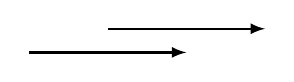
\begin{tikzpicture}[>=\ReadArrowType]
				\draw[->,style=thick] (0,0) -- (2,0);
				\draw[->,style=thick] (1.0,0.3) -- (3.0,0.3);
			\end{tikzpicture}

			\vspace{3mm}
			or (symmetrically)
			\vspace{3mm}

			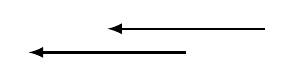
\begin{tikzpicture}[>=\ReadArrowType]
				\draw[->,style=thick] (2,0) -- (0,0);
				\draw[->,style=thick] (3.0,0.3) -- (1.0,0.3);
			\end{tikzpicture}
		\end{center}
	\vspace{0.5cm}
	\item ``Innie'' overlap
		\begin{center}
			\vspace{-0.5cm}
			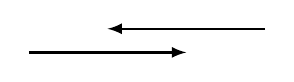
\begin{tikzpicture}[>=\ReadArrowType]
				\draw[->,style=thick] (0,0) -- (2,0);
				\draw[->,style=thick] (3,0.3) -- (1,0.3);
		\end{tikzpicture} \end{center}
	\vspace{0.5cm}
	\item ``Outie'' overlap
		\begin{center}
		\vspace{-0.5cm}
		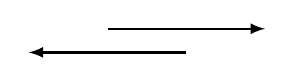
\begin{tikzpicture}[>=\ReadArrowType]
				\draw[->,style=thick] (2,0) -- (0,0);
				\draw[->,style=thick] (1.0,0.3) -- (3.0,0.3);
		\end{tikzpicture} \end{center}
\end{enumerate}

Now that we've formalized the definition of an overlap, what we'd like to do is
compute 

\section{Building the fragment string assembly graph}


\section*{Acknowledgments}

Acknowledgements

\bibliographystyle{plain}
\bibliography{refs}

\end{document}
